\documentclass[11pt]{beamer}
\usepackage[utf8]{inputenc}
\usepackage[T1]{fontenc}
\usepackage{lmodern}
\usepackage{xcolor}
\usetheme{Hannover}
\usepackage{multirow}
\usepackage{amssymb} 
\usepackage{amsmath}
\usepackage{graphicx}
\usepackage{tikz}
%\NewDocumentCommand\DownArrow{O{2.0ex} O{black}}{%
%	\mathrel{\tikz[baseline] \draw [<-, line width=1.5pt, #2] (0,0) -- ++(0,#1);}
%}
\begin{document}
	\author{Ashim Khadka}
	\title{Introduction to LaTex}
	%\subtitle{}
	%\logo{}
	\institute{Gandakai College of Engineering and Science}
	\date{\today}
	%\subject{}
	%\setbeamercovered{transparent}
	%\setbeamertemplate{navigation symbols}{}
	\begin{frame}[plain]
		\maketitle
	\end{frame}
	\begin{frame}{Outline}
		\tableofcontents
	\end{frame}
	\section{Introduction}
	\begin{frame}{}
		\begin{center}
			\huge Introduction
		\end{center}
	\end{frame}
	\begin{frame}{LaTex}
		\begin{itemize}
			\only<1->{
				\item LaTeX is a software for typesetting documents
				\begin{itemize}
					\item It's a document preparation system
				\end{itemize}
			}
			\only<2->{
				\begin{figure}
					\centering
					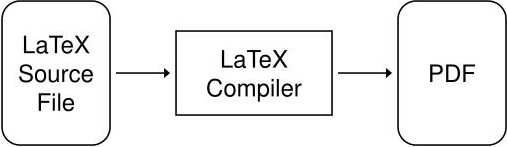
\includegraphics[width=0.7\linewidth]{Images/what-is-latex}
					\caption{What is latex?}
					\label{fig:what-is-latex}
				\end{figure}
			}
			\item<3-> LaTeX is a free, open source software
			\only<4->{
				\item LaTeX is especially well-suited for scientific and technical documents
				\begin{itemize}
					\item Superior typesetting of mathematical formulas is legendary
					\item Cross-referencing capabilities
				\end{itemize}
			}
		\end{itemize}
	\end{frame}
	\begin{frame}{Comparison}		
		\begin{figure}
			\centering
			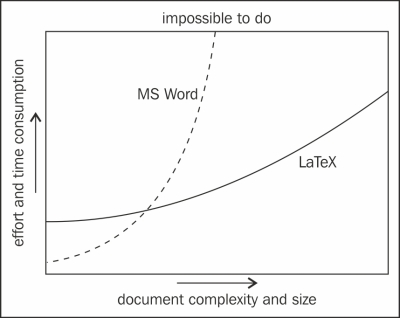
\includegraphics[width=0.7\linewidth]{Images/complexity_latex}
			\caption{Using LaTeX on Windows by Marko Pinteric (www.pinteric.com/miktex.html)}
			\label{fig:complexitylatex}
		\end{figure}
	\end{frame}
	\begin{frame}{How to use LaTex?}
		\begin{tabular}{lll}
			\hline
			\textcolor{red}{LOCALLY}&  &   \textcolor{red}{REMOTELY}   \\
			\begin{tabular}{@{}l@{}}Need to install Tex \\ Distribution \& Editor\end{tabular} &  &   No installation required   \\
			Windows OS:& \begin{tabular}{@{}l@{}}\textbf{TeXLive} \\  \textbf{MiKTeX}\end{tabular}  &   \textbf{Overleaf}   \\
			
			Editors:& \begin{tabular}{@{}l@{}l@{}}\textbf{Texstudio}\\ \textbf{TeXnicCenter} \\ \textbf{TeXmaker}\end{tabular} &   www.overleaf.com \\
			
			Mac OS:& \begin{tabular}{@{}l@{}}\textbf{MacTeX}\\ \textbf{MiKTeX} \end{tabular} &    \\
			
			Editors:& \begin{tabular}{@{}l@{}}\textbf{Texstudio}\\ \textbf{TeXmaker} \end{tabular}&   \\
			\hline
		\end{tabular}
	\end{frame}
	\begin{frame}{Why use LaTex?}
		\begin{itemize}
			\item Free: Open Source
			\item Looks better
			\begin{itemize}
				\item Especially math
			\end{itemize}
			\item Separation of content \& formatting
			\item More flexible
			\item Easier concurrent editing
			\item Easier citations
		\end{itemize}
	\end{frame}
	\subsection{Create Document}
	\begin{frame}{}
		\begin{center}
			\huge Create Document
		\end{center}
	\end{frame}
	\begin{frame}{Creating Document}
		\begin{enumerate}
			\item Launch the \textbf{LaTeX editor}: Click on the \textbf{New} button
			\item Enter the following lines:
			\begin{itemize}
				\item[]<1->\textbackslash\textit{documentclass\{article\}}
				\item[]<2->\textbackslash\textit{begin\{document\}}
				\begin{itemize}
					\item[]<3-> This is our first document.
				\end{itemize}
				\item[]<2->\textbackslash\textit{end\{document\}}
			\end{itemize}
			\item<4-> Click on the \textbf{Save} button and save the document
			\item<5-> Click on the \textbf{Build \& Run} or \textbf{Typeset} button
		\end{enumerate}		
	\end{frame}
	\begin{frame}{Modify Document}
		\begin{itemize}
			\item[]\textbackslash\textit{documentclass[a4paper,11pt]\{article\}}
			\item[]\textbackslash\textit{begin\{document\}}
			\begin{itemize}
				\item[]\textbackslash\textit{title\{Example 2\}}
				\item[]\textbackslash\textit{author\{My name\}}
				\item[]\textbackslash\textit{date\{February 6, 2021\}} or \textbackslash\textit{date\{\textbackslash today\}}
				\item[]\textbackslash\textit{maketitle}
				\item[]\textbackslash\textit{section\{Introduction\}}
				\item[] This is our first document.
				\item[]\textbackslash\textit{subsection\{GCES\}}
				\item[] Gandaki college of engineering and science
			\end{itemize}
			\item[]\textbackslash\textit{end\{document\}}
		\end{itemize}		
	\end{frame}
	\section{Latex Writing}
	\begin{frame}{}
		\begin{center}
			\huge {Latex Writing}
		\end{center}
	\end{frame}
	\begin{frame}{Latex Writing}
		\begin{itemize}
			\item Creating Lists
			\item Inserting Figures
			\item Creating Column
			\item Typing Math Formulas
		\end{itemize}
	\end{frame}
	\begin{frame}{}
		\begin{center}
			\huge {Creating Lists}
		\end{center}	
	\end{frame}
	\begin{frame}{Creating Lists}
		\begin{itemize}
			\item Arranging text in the form of a list can be very reader-friendly
			\item Present several ideas by a clear structure which is easy to survey
			\begin{enumerate}
				\item Bulleted lists
				\item Numbered lists
				\item Definition lists
			\end{enumerate}
		\end{itemize}
	\end{frame}
	\begin{frame}{Example: Creating Lists}
		\begin{columns}
			\column{0.5\textwidth}
			\begin{itemize}
				\item[] \textbackslash begin\{itemize\}
				\item[] \textbackslash item Bulleted lists
				\item[] \textbackslash begin\{enumerate\}[I]
				\item[] \textbackslash item Hello
				\item[] \textbackslash end\{enumerate\} 
				\item[] \textbackslash item Numbered lists
				\item[] \textbackslash item Definition lists
				\item[] \textbackslash end\{itemize\}
			\end{itemize}	
			\column{0.5\textwidth}
			\begin{itemize}
				\item[] \textbackslash begin\{enumerate\}
				\item[] \textbackslash item Bulleted lists
				\item[] \textbackslash begin\{enumerate\}[a]
				\item[] \textbackslash item Hello
				\item[] \textbackslash end\{enumerate\} 
				\item[] \textbackslash item Numbered lists
				\item[] \textbackslash item Definition lists
				\item[] \textbackslash end\{enumerate\}
			\end{itemize}	
		\end{columns}		
		\begin{figure}
			\centering
			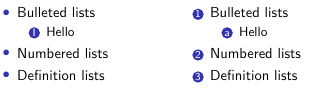
\includegraphics[width=0.7\linewidth]{Images/Lisiting}
			\caption{Listing}
			\label{fig:listing}
		\end{figure}
	\end{frame}
	\begin{frame}{}
		\begin{center}
			\huge {Inserting Figure}
		\end{center}	
	\end{frame}
	\begin{frame}{Inserting Figure}
		Visual representation
		\begin{itemize}
			\item[] \textbackslash \textit{begin\{figure\}}
			\part{title}		\item[] \textbackslash \textit{centering}
			\item[] \textbackslash \textit{includegraphics[width=0.7\textbackslash linewidth]\{what-is-latex\}}
			\item[] \textbackslash \textit{caption\{What is Latex?\}}
			\item[] \textbackslash \textit{label\{fig:what-is-latex\}}
			\item[] \textbackslash \textit{end\{figure\}} 
		\end{itemize}
		\begin{figure}
			\centering
			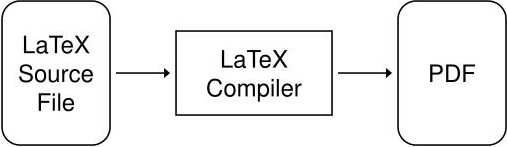
\includegraphics[width=0.7\linewidth]{Images/what-is-latex}
			\caption{What is Latex?}
			\label{fig:what-is-latex1}
		\end{figure}
	\end{frame}
	%\section{Creating Column}
	\begin{frame}{}
		\begin{center}
			\huge {Creating Column}
		\end{center}	
	\end{frame}
	\begin{frame}{Creating Column}
		Representation document in column
		\begin{itemize}
			\item[] \textbackslash \textit{begin\{columns\}}
			\item[] \textbackslash \textit{column\{0.4\textbackslash textwidth\}}
			\item[] Hi
			\item[] \textbackslash \textit{column\{0.4\textbackslash textwidth\}}
			\item[] Hello
			\item[] \textbackslash \textit{end\{columns\}} 
		\end{itemize}
		\begin{columns}
			\column{0.4\textwidth}
			Hi
			\column{0.6\textwidth}
			Hello
		\end{columns}
	\end{frame}
	\begin{frame}{}
		\begin{center}
			\huge {Typing Mathematics Formulas}
		\end{center}	
	\end{frame}
	\begin{frame}{Typing Mathematics Formulas}
		\begin{itemize}
			\item LaTeX offers excellent quality for mathematical typesetting
			\item \textbackslash usepackage\{amssymb\} 
			\item \textbackslash usepackage\{amsmath\}
		\end{itemize}
		\pause
		$x^2+\underset{\theta \rightarrow 0}{lim} \frac{\sin x}{x}$
		\begin{itemize}
			\item[]  \$expression\$
			\item[] \{expression\}\_\{subscript\}
			\item[] \{expression\}\string ^\{superscript\}
			\item[] \textbackslash sqrt[order]\{value\}
			\item[] \textbackslash frac\{numerator\}\{denumerator\}
			\item[] \textbackslash begin\{align\}
			\item[]	x+y
			\item[]	\textbackslash label\{math\}
			\item[] \textbackslash end\{align\}
		\end{itemize}
		From (\ref{eq:math})
		\begin{align}
			x^2+\underset{\theta \rightarrow 0}{lim} \frac{\sin x}{x}
			\label{eq:math}
		\end{align}
	\end{frame}
	%\section{Referring to a key}
	\begin{frame}{Referring to a key}
		\only<1>{
			\begin{block}{Assigning a key}
				\begin{itemize}
					\item Command \textbackslash label\{name\} assigns the current position to the key name 
					\item Figure:  \textbackslash label\{fig:name\} Figure  \textbackslash label\{eq:name\} 
				\end{itemize}		
			\end{block}
		}
		\only<2>{
			\begin{itemize}
				\item Once a label has been set and given a name
				\item \textbackslash ref\{name\}: From (\ref{eq:math})(\textbackslash ref\{eq:math\})
			\end{itemize}
		}
	\end{frame}
	\section{Presentation}
	\begin{frame}{}
		\begin{center}
			\huge {Presentation: Beamer}
		\end{center}	
	\end{frame}
	\begin{frame}{Presentation: Beamer}
		\begin{itemize}
			\item Beamer is a powerful and flexible LaTeX class to create great looking presentations
			\item This article outlines the basis steps to making a Beamer slideshow:
			\begin{itemize}
				\item creating the title page
				\item highlighting important points
				\item making a table of contents and adding effects to the slideshow
			\end{itemize}
		\end{itemize}
	\end{frame}
\end{document}